\chapter{Entrepreneurs Guide To Start and Scale Any Business}

This chapter follows a School of Hard Knocks conversation with Chris Meroff, curated for this volume by LazyingArt LLC. We begin with a teaser about professional athletes and marketing, but the real work of the lecture is slower and more deliberate: first establish entrepreneurial scale, then identify a concrete problem, then test ideas against failure, sales, geography, and finally the founder's own tendency to become the bottleneck. The mathematics here is necessarily light and mostly reconstructed from the transcript, but there is still a clear quantitative spine: repeated conversations, bounded markets, capital loss, and throughput.

\section{Teaser and Entrepreneurial Baseline}

The lecture opens out of order, with a payoff before the argument: a physical therapy business is now attracting professional athletes from the major sports leagues, and we are told that this is ``the key to marketing.'' That line is not yet explained. It functions the way a good opening move should function: it creates a future point that the rest of the chapter must earn.

Then the chronology resets. Meroff is introduced as a serial entrepreneur with about a dozen businesses. His first business began in 1996 with his parents, when he was twenty-two, and it was sold only recently. The early company was not a vague side hustle; it consulted for public schools and helped bring dollars back for services for students with special needs. We therefore get three pieces of grounding at once: duration, domain seriousness, and a long enough sample of decisions that the later judgments about success and failure are worth hearing.

\paragraph{Anecdote.}
The first company is family-linked, mission-linked, and very old by startup standards.

\paragraph{Claim.}
The chapter is not about a single lucky venture. It is about a durable way of thinking across many ventures.

\paragraph{Mechanism.}
The host first secures the speaker's time horizon and track record, and only then asks for principles.

\section{The First Leap: Leaving Safety for a Larger Market}

When asked for the best financial decision of his life, Meroff does not point to a complicated acquisition structure or a clever financing maneuver. He points instead to a directional commitment. He could have stayed inside the safe orbit of a family business that already worked. Instead he moved to another state, where he knew nobody, expected to lose money in the first year, and trusted that the same product and service would behave differently in a larger market.

The important rhythm here is that the lecture shifts from biography to risk. Entrepreneurship is not introduced as branding, content, or social media tactics. It begins with willingness to enter uncertainty in a place where one has no network and no guarantee of immediate reward. That is why this section must remain near the beginning of the chapter: the later arguments about marketing and scaling only make sense after we have seen that the speaker regards short-run discomfort as the price of discovering whether a larger market exists.

What matters is not blind optimism. What matters is the combination of two beliefs: that the product is real, and that the market is larger than the founder's current comfort zone. The lecture's later insistence on sales evidence is already latent here. One makes the leap, but one does not worship the leap. One jumps in order to learn what the larger market will actually say.

\section{ROI Physical Therapy: Problem Before Brand}

The first detailed business story is ROI Physical Therapy, and the lecture handles it in the right order. We do not begin with the brand name or the facility size. We begin with a broken knee. Meroff describes injuring himself badly in a tournament with his nephews: torn ACL, torn MCL, fractured patella, torn meniscus. He then moves through the existing system and finds the thing that matters for the chapter: in that system, one becomes ``just a number.''

\paragraph{Anecdote.}
A serious sports injury becomes the source of a business idea.

\paragraph{Claim.}
The problem was not merely that bodies needed repair. The problem was that the system treated the patient as a broken part rather than as a whole athlete.

\paragraph{Mechanism.}
The business recruits physical therapists into a larger mission. They are not serving a machine; they are serving a person.

We may summarize the operating idea schematically as
\begin{equation}
\text{care}
=
\text{repair of injury}
+
\text{psychology}
+
\text{nutrition}
+
\text{massage}
+\cdots
\end{equation}
This equation is not stated in the lecture in symbolic form, but it captures the business logic exactly: the service is widened until it addresses the whole athlete rather than only the visibly broken component.

This widening is not cosmetic. It changes both the customer offer and the labor offer. For the customer, the promise becomes richer than standard treatment. For the therapists, the work becomes ``something bigger to shoot for.'' In the lecture's sequence, that is the crucial middle term between problem recognition and scale. The business does not merely solve a need; it assembles a team around a more ambitious description of the need.

The later payoff then arrives: a $7{,}000$ square foot facility in a sports arena, and professional athletes coming in from the NBA, NFL, Major League Baseball, and NHL. The opening teaser is thus no longer a slogan. It is the end of a chain:
\[
\text{felt problem}
\longrightarrow
\text{richer service model}
\longrightarrow
\text{team buy-in}
\longrightarrow
\text{market credibility}.
\]

\section{Failure, Validation, and the Discipline of Sales}

After the success story, the lecture makes a necessary turn. The host asks for the worst financial decision, and the atmosphere changes immediately. Failure is not treated as a blemish to be hidden; it is treated as part of the game. The more precise warning is stronger than the generic slogan about failure. The true danger is not that one idea fails. The true danger is that one continues feeding capital to an idea after the evidence has turned against it.

\paragraph{Anecdote.}
An investment made in 2019 did not work. The pandemic shut it down. Later, instead of burying the idea, Meroff tried to resurrect it so as not to ``lose all this money.''

\paragraph{Claim.}
That resurrection was the deeper error.

\paragraph{Mechanism.}
The founder tried to rescue sunk cost with fresh cost.

If we write the capital damage in the lecture's own rough numbers, we obtain
\begin{equation}
L_{\text{total}}
\approx
L_{\text{early stop}} + L_{\text{revival}}
\approx
\text{\$}1{,}000{,}000 + \text{\$}1{,}000{,}000
\approx
\text{\$}2{,}000{,}000.
\end{equation}
Again, this is transcript-backed arithmetic, not a board-derived formula. But it gives us a clean way to state the point: the cost of refusing to accept a bad idea can be of the same order as the cost of the original failure.

\subsection{Question \& Answer}

The lecture now raises its sharpest question: how do we know whether an idea is actually good?

The answer is intentionally brutal. Not passion. Not elegance. Not the pitch. Sales.

\begin{definition}
Let $C$ denote serious conversations with the market, and let $S$ denote realized sales. The lecture's validation rule is that the market must answer. In compressed form,
\begin{equation}
\text{idea validation} \Rightarrow S>0.
\end{equation}
\end{definition}

The point of the symbol is not to claim that one sale proves a great company. The point is to preserve the lecture's hierarchy of evidence. Before sales, the founder's certainty is weak evidence. After sales, one may argue about scale, margins, channel, and repetition. But before sales, the idea has not yet crossed the first gate.

Meroff then gives a rough threshold: he wants at least a thousand conversations before deciding that the market has answered in a reliable way. Let
\begin{equation}
C_{\min}=1000,
\qquad
T \approx 6 \text{ months}.
\end{equation}
A useful editorial unpacking is
\begin{align}
\frac{C_{\min}}{T}
&\approx
\frac{1000}{6}
\approx
167
\qquad \text{conversations per month},\\
\frac{1000}{26}
&\approx
38
\qquad \text{conversations per week},\\
\frac{1000}{180}
&\approx
5.6
\qquad \text{conversations per day}.
\end{align}

\begin{remark}
These rates are not spoken calculations from the lecture. They are a faithful reconstruction of the speaker's practical point: the intimidating total becomes manageable when spread across time.
\end{remark}

What we should preserve in the notes is the structure of the answer. First, a bad resurrection teaches that desire is not evidence. Second, sales are the operative indicator. Third, the founder should expose the idea to repeated contact with the market until the answer is no longer a projection of the founder's own enthusiasm.

\section{New Industries, Expert Partners, and Mentors}

Only after the validation segment does the lecture move to Coffee and Crisp. This order matters. The coffee business is not introduced as a dream project floating above business law. It arrives after the rules of validation have been stated. Meroff says he loves coffee and community, and wanted to create a place where people gather around something he himself enjoys. That gives the origin story warmth, but the lecture immediately stabilizes it with a second principle: when entering a new industry, he looks for experts who are deeply passionate about the product or service itself.

The structure is therefore paired:
\[
\text{business drive} + \text{domain passion}.
\]
The notation is schematic, but the idea is precise. He does not insist that the same person carry all kinds of competence. He can bring intensity around business; someone else may bring intensity around the product. That principle, he says, is how one gets from coffee shops to a record label without pretending that all expertise originates in the founder.

The mentor discussion deepens the same logic. Early on, he did not even plan to find a mentor. He stumbled into one soon after moving, heard a story that sounded like genuine business knowledge, and accepted guidance. The lecture does not present mentorship as a sentimental accessory. It is another instance of a more general rule: one scales by admitting that intelligence and clarity may live outside the founder.

\section{Local Marketing as a Geometric Problem}

From experts and mentors the lecture turns outward, to awareness. The host asks how a person with an idea, perhaps even without much capital, should generate proof of concept. Meroff's answer begins with networking. He treats networking not as optional polish, but as a major share of the work. One must become known.

The restaurant example then specializes the point. Here the lecture becomes almost geometric. A restaurant is ``very geographically centered.'' People do not travel indefinitely far each day for a meal, so the relevant audience is local. The lecture speaks colloquially of taking a circumference around the restaurant and hitting every door one can find. We should not take the geometry too literally, but it is still useful to write the local market as
\begin{equation}
\mathcal{A}(r)=\{x:d(x,x_0)\le r\},
\end{equation}
where $x_0$ is the restaurant location and $r$ is a practical daily radius inside which customer acquisition is plausible.

\begin{figure}[h]
\centering
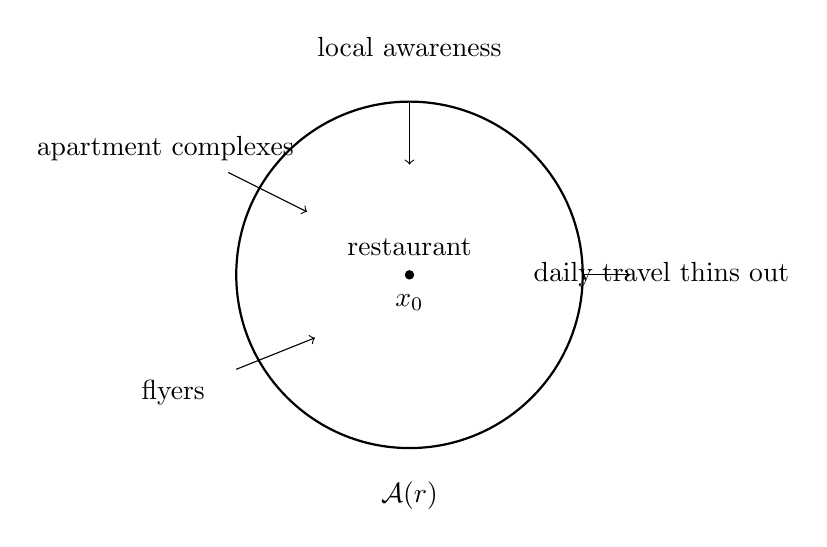
\begin{tikzpicture}[scale=1.0]
\draw[thick] (0,0) circle (2.2);
\fill (0,0) circle (0.06);
\node at (0,0.35) {restaurant};
\node at (0,-0.35) {$x_0$};

\node at (-3.1,1.6) {apartment complexes};
\draw[->] (-2.3,1.3) -- (-1.3,0.8);

\node at (-3.0,-1.5) {flyers};
\draw[->] (-2.2,-1.2) -- (-1.2,-0.8);

\node at (0,2.9) {local awareness};
\draw[->] (0,2.2) -- (0,1.4);

\node at (3.2,0.0) {daily travel thins out};
\draw[->] (2.2,0) -- (2.8,0);

\node at (0,-2.8) {$\mathcal{A}(r)$};
\end{tikzpicture}
\caption{A transcript-backed sketch of local restaurant marketing as a bounded catchment problem. The lecture's ``circumference'' language is practical rather than literally Euclidean, but the picture clarifies the idea.}
\end{figure}

Now the lecture tightens its definition of marketing. Marketing is not applause. Marketing is not a good-looking plan. Marketing is what generates sales. Thus the test becomes instrumental:
\[
\text{marketing plan works}
\Rightarrow
\uparrow S
\quad \text{inside the intended market.}
\]
If sales do not rise where they should rise, then the lecture's instruction is severe and clean: discard the plan and start over.

The sequence here is worth preserving exactly. First identify who needs to hear about the offer. Then create as many channels as possible---print, digital, in-person---through which that audience can become aware that they are, in fact, the ideal client.

\section{Pride, Bottlenecks, and the Purpose Statement}

The host next asks for the biggest challenge of being a business owner. Meroff answers with a move inward: pride. That answer is stronger than it first appears. Pride means centralization. The founder solves all the problems, manages all the crises, processes all the information, and gradually trains the organization to wait.

A compact way to represent the lecture's bottleneck logic is
\begin{equation}
Q = \min\!\bigl(Q_{\text{founder}},Q_{\text{team}}\bigr),
\end{equation}
where $Q$ is actual organizational throughput, $Q_{\text{founder}}$ is the rate at which the founder can absorb and resolve problems, and $Q_{\text{team}}$ is the latent capacity of the broader organization. If all roads must pass through the founder, the system never exceeds the founder.

\subsection{Question \& Answer}

What, then, actually blocks scale inside the founder?

The lecture's answer is that pride produces silence. Because the founder is good at solving problems quickly, everyone else learns not to own solutions. The organization becomes dependent. To scale, the founder must stop treating himself as the unique processing unit. He must listen, and he must permit other people to own the answer to the problem rather than merely reporting the problem upward.

This interior diagnosis then turns back outward into the final marketing doctrine. Marketing, we are told, begins with the product or problem being solved. Once that is clearly defined, the firm creates a purpose statement. We may write the lecture's closing sequence as
\begin{equation}
P
\longrightarrow
\text{story}
\longrightarrow
A
\longrightarrow
S,
\end{equation}
where $P$ is the purpose statement, $A$ is the audience, and $S$ is sales.

\begin{definition}
A purpose statement is the compact internal formulation of what problem the company is solving and what story the company is prepared to tell about that problem.
\end{definition}

The lecture adds two important constraints. First, the story changes as the market changes. Second, the story must be bought into by the organization itself before the firm obsesses over website polish or content volume. This is how the lecture closes the loop to its opening teaser. The attracting of elite clients is not magic. It is the far downstream consequence of a chain that begins with problem clarity and ends with coordinated storytelling to the right audience.

\section{Summary}

We can now see the architecture of the lecture clearly. It begins with an outcome---professional athletes and marketing---and then reconstructs the path to that outcome through a sequence of disciplined moves. First, accept uncertainty in pursuit of a larger market. Second, build from a real problem rather than a decorative brand. Third, let failure teach the cost of ignoring evidence. Fourth, treat sales and repeated market conversations as the first serious test of an idea. Fifth, borrow expertise through partners and mentors. Sixth, understand that some markets are local and must be saturated locally. Finally, recognize that the founder's own pride can throttle scale unless the organization is aligned around a purpose statement and a shared story.

The chapter is therefore not a catalogue of startup tips. It is a model of entrepreneurial reasoning under constraint. One begins with a problem, exposes the idea to the market, localizes the audience where necessary, and refuses to let the founder's ego stand where the organization's throughput should be.